\documentclass{article}
\usepackage[UTF8]{ctex}
\usepackage{amsmath}
\usepackage{amssymb}
\usepackage{graphicx}
\usepackage{float}
\usepackage{datetime}
\usepackage{geometry}

\geometry{a4paper, top=2.54cm, bottom=2.54cm, left=3.18cm, right=3.18cm}

\author{刘思昀 SLST 2022522011}

\title{General Physics II 制流和分压电路的研究}

\begin{document}

\date{\formatdate{20}{3}{2024}}

\maketitle

\section{制流电路}
\subsection{原理与步骤}

\begin{figure*}[htbp]
    \centering
    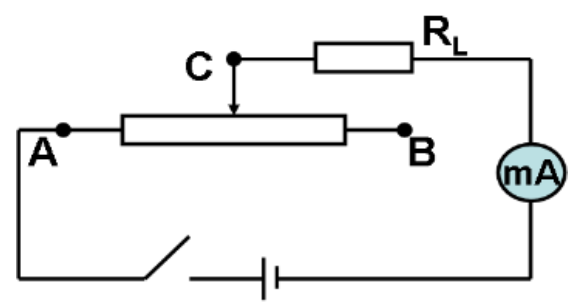
\includegraphics[width=0.5\textwidth]{current-control.png}
    \caption{制流电路实验电路图}
\end{figure*}

直流电源输入电压 $E = 1.5 A$

固定$\beta$值,调节电位器从而改变$K$值,记录电流表的示数$I$

\subsection{实验数据及数据处理}
电位器旋至最大值时(该实验中取g刻度位置为电位器阻值最大值),此时电流表示数记为$I_{max}$,以此对于相同$\beta$值时的电流表示数进行归一化处理。

注:$\beta = 98.3824, K = 0.0217$时(图2中标红处),此处实验数据为异常值,根据此处代表的物理意义,在绘图时替换为$1.00000$

\begin{align*}
    \beta &= \frac{R_L}{R_0} \\
    K &= \frac{R_{ac}}{R_0} \\
    Y &= \frac{I}{I_{max}}
\end{align*}

\begin{figure*}[htbp]
    \centering
    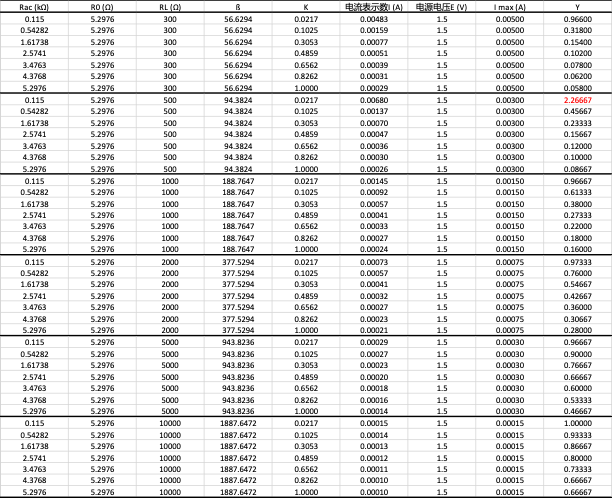
\includegraphics[width=0.9\textwidth]{current-control-data.png}
    \caption{制流电路实验数据}
\end{figure*}

\begin{figure*}[htbp]
    \centering
    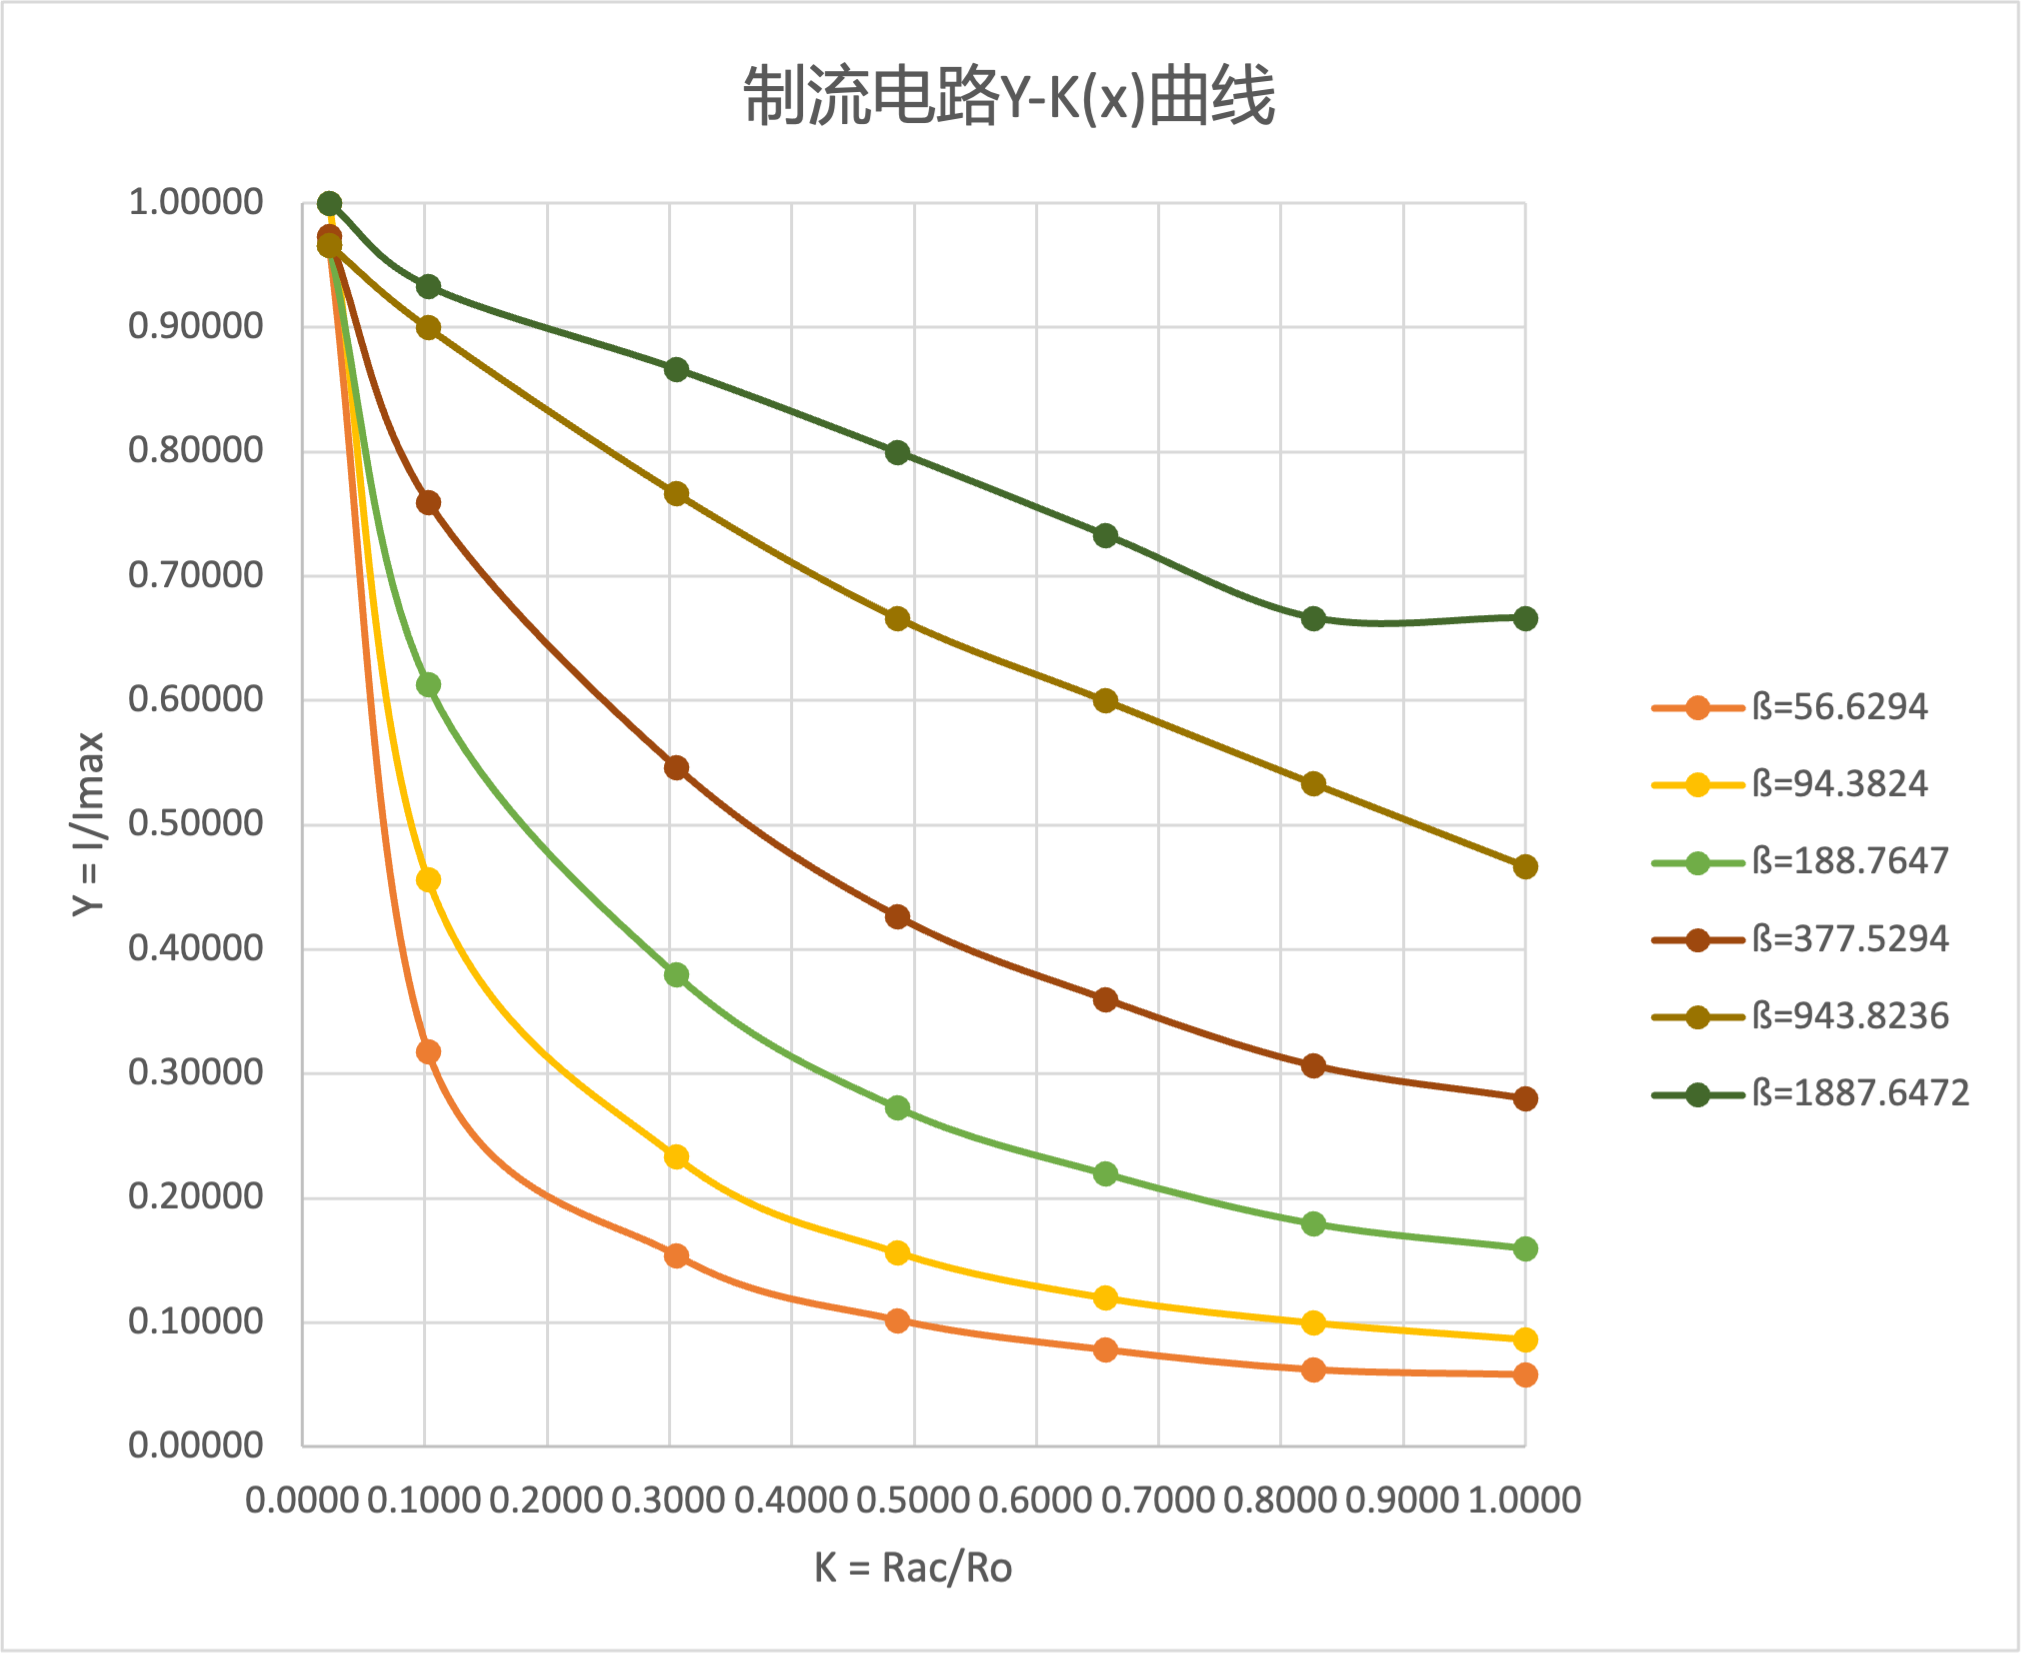
\includegraphics[width=0.9\textwidth]{current-control-plot.png}
    \caption{制流电路不同$\beta$值下$Y-K$曲线}
\end{figure*}

\newpage

\subsection{结论}
由图线可知:

\begin{itemize}
    \item $\beta$越大,电流调节范围越小
    \item $\beta \geq 1$时,调节的线性较好
    \item $\beta$较小,即$R_0 \gg R_L$时,$\beta$接近0时电流变化很大,细调程度差
    \item 不论$R_0$大小如何,负载上通过的电流都不可能为0
\end{itemize}

\section{分压电路}
\subsection{原理与步骤}

\begin{figure*}[htbp]
    \centering
    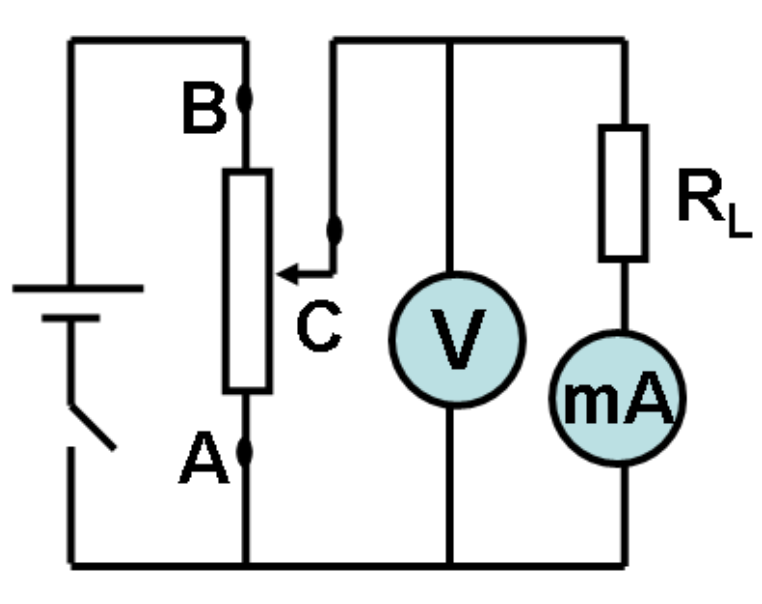
\includegraphics[width=0.5\textwidth]{voltage-control.png}
    \caption{分压电路实验电路图}
\end{figure*}

直流电源输入电压 $E = 1.5 A$

固定$\beta$值,调节电位器从而改变$K$值,记录电压表的示数$I$

\subsection{实验数据及数据处理}
电位器旋至最大值时(该实验中旋钮最大位置为电位器阻值最大值),以此对于相同$\beta$值时的$R_{ac}$阻值进行归一化处理。

\begin{align*}
    \beta &= \frac{R_L}{R_0} \\
    K &= \frac{R_{ac}}{R_0} \\
    Y &= \frac{U_{L}}{E}
\end{align*}

\begin{figure*}[htbp]
    \centering
    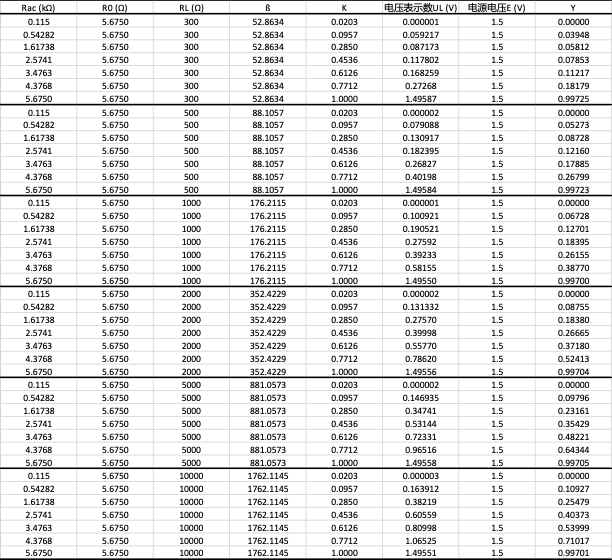
\includegraphics[width=0.8\textwidth]{voltage-control-data.png}
    \caption{分压电路实验数据}
\end{figure*}

\begin{figure*}[htbp]
    \centering
    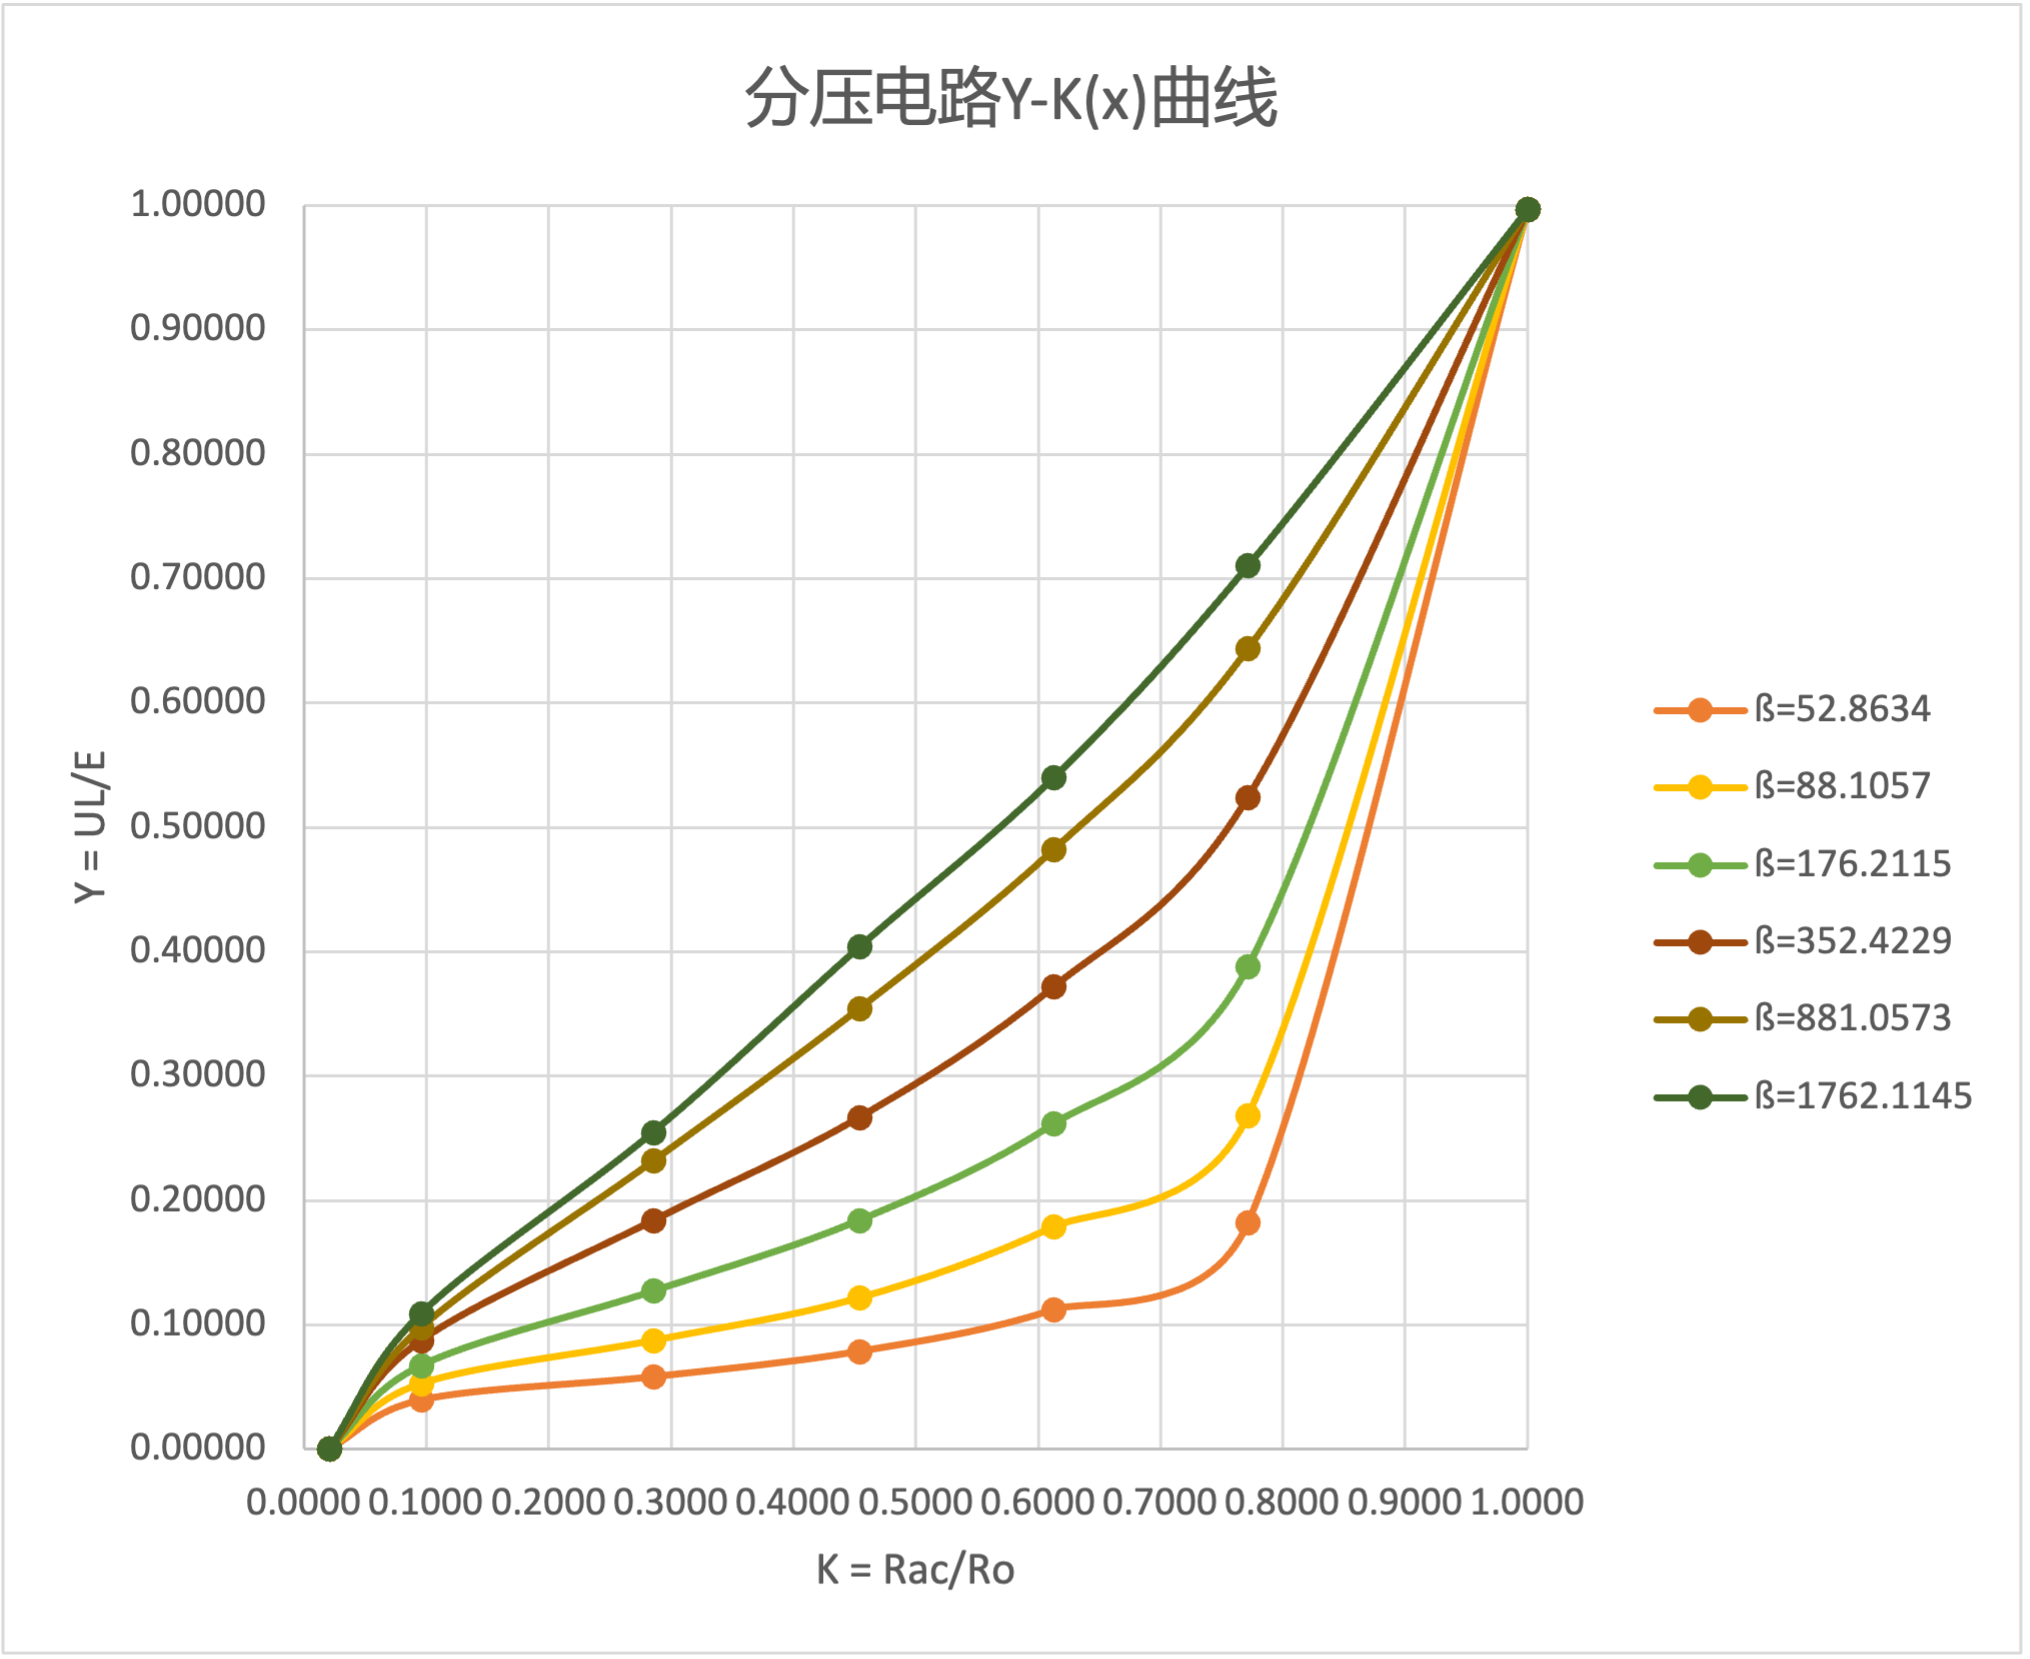
\includegraphics[width=0.9\textwidth]{voltage-control-plot.png}
    \caption{分压电路不同$\beta$值下$Y-K$曲线}
\end{figure*}

\subsection{结论}
由图线可知:

\begin{itemize}
    \item $\beta$越大,调节越均匀
    \item $\beta$越大,变阻器上消耗的电能越大
\end{itemize}

\section{思考题}
\subsection{如图1,现可变电阻的 B、C 端未接一根线能起到制流的作用,若在 B、C端上接一根线也能起到制流的作用,则两种接线方式有什么不同?对实验的过程和结果会有什么影响?}

$\romannumeral1$. 电流仍然可以通过改变A到B的阻值来控制,但电流的控制范围会减小,因为总是有一部分电流通过BC导线。

$\romannumeral2$. 电流表将显示流过$R_L$和BC导线的总电流,但由于BC导线的低阻抗,这可能导致测量的电流大于仅通过可变电阻时的电流。

$\romannumeral3$. 由于BC并联路径的存在,AB部分的可变电阻将不再是控制电流的唯一手段,这可能使得对电流的精确控制变得更加困难。

\subsection{制流电路与分压电路有何相同之处,又有何不同之处?}

相同之处:

$\romannumeral1$. 两者都利用了电阻的特性来实现电路中电流或电压的控制。

$\romannumeral2$. 都可以通过调节可变电阻的阻值来改变电路的工作状态。

不同之处:

$\romannumeral1$. 制流电路主要用于控制流经电路的电流大小。在这种电路中,可变电阻与负载电阻串联,通过改变可变电阻的阻值来改变电路的总电阻,从而调节电流的大小。制流电路的电流范围从$I_{min}$到$I_{max}$,但不可能调节到零,只能使电流在一定范围内变化。

$\romannumeral2$. 分压电路则主要用于控制负载两端的电压大小。在这种电路中,可变电阻和负载电阻形成分压器,可变电阻的阻值改变将导致负载两端电压的变化。分压电路可以调节的电压范围为0到电源电压$E$,即$U_L$的范围是0到$E$。 

$\romannumeral3$. 在制流电路中,负载电阻上的电流值取决于电源电压和电路的总阻值,而在分压电路中,负载电阻两端的电压取决于电源电压和电阻比率。

$\romannumeral4$. 制流电路适合需要稳定电流的场合,比如驱动LED或电动机。分压电路则适用于需要特定电压的场合,如给传感器提供参考电压。

\subsection{分析制流电路或分压电路中的$Y-K(x)$关系有何作用?}

在制流电路或分压电路中,$Y$通常表示输出比例,而$K(x)$表示可变电阻器上电阻比例,即可变电阻器的阻值与其最大可能阻值的比例。

分析$Y-K(x)$关系的作用如下:

$\romannumeral1$. 通过这个关系,可以了解在调节可变电阻器的阻值时,输出的电流或电压将如何变化。

$\romannumeral2$. 有助于决定应使用何种电阻和电阻的最大、最小值,以便在特定的应用中得到期望的调节范围和精度。

$\romannumeral3$. 在某些应用中,希望调节过程具有良好的线性度,即阻值的增加或减少将导致电流或电压成比例地变化。$Y-K(x)$图能显示出电路的线性度,帮助识别在哪个阻值范围内输出比例变化最为线性。

$\romannumeral4$. 在分压电路中,通过分析$Y-K(x)$关系,可以评估变阻器上消耗的能量,并尽可能地减少功耗。

$\romannumeral5$. 如果实际的$Y-K(x)$曲线与预期的有偏差,这可能表明电路中存在元件损坏或连接错误等问题。因此,这个关系也可以用于故障诊断和故障分析。

\subsection{如何运用分压原理,从 1.5 伏的电源电压中分出千分之一的结果?(写出实际可行的方案)}

要从1.5伏的电源中分出千分之一的电压,即要得到1.5毫伏的电压,可以通过一个分压电路实现。分压电路通常由两个电阻串联组成,并从它们的连接点取电压。分出的电压与这两个电阻的比值成正比。为了得到千分之一的电压,电阻之间的比值应该是$999:1$。

这里是一个具体的方案:

1. 选择电阻值,这里选择$1 \Omega$和$999 \Omega$

2. 将两个电阻串联连接后,连接到$1.5 V$的电源上。

3. 从$1 \Omega$电阻的两端取电压,可以得到$1.5 mV$

\section{分析与讨论}
\begin{itemize}
    \item 实验时需要时刻注意直流电源是否保持$1.5 V$左右的电压输出,确保其没有突然调至0,否则会对实验数据产生影响
    \item 实验开始前要对电位器的各个档位的阻值进行定标
    \item 调整电位器刻度时,尽可能从竖直上方观察,尽可能保证每次调节在同一个位置上
    \item 并联电路连接时可以一个回路一个回路连接,不易出错
\end{itemize}

\end{document}